\subsection{Etap Operate}
Faza operacyjna (\textit{Operate}) obejmuje utrzymanie aplikacji w~środowisku produkcyjnym oraz zarządzanie usługami wspierającymi (bazami danych, brokerami wiadomości).
Strukturę utrzymywanego środowiska przedstawia rysunek~\ref{fig:infrastructure}: cztery przestrzenie nazw (ang. \textit{namespace}) klastra pełnią cztery odrębne role --- platformową (\texttt{kube-system}: Traefik jako jedyny punkt wejścia HTTP oraz kontroler Sealed Secrets), dostarczania (\texttt{argocd}), aplikacyjną (\texttt{bsc-devops}) i~obserwacyjną (\texttt{observability}).

\begin{figure}[H]
    \centering
    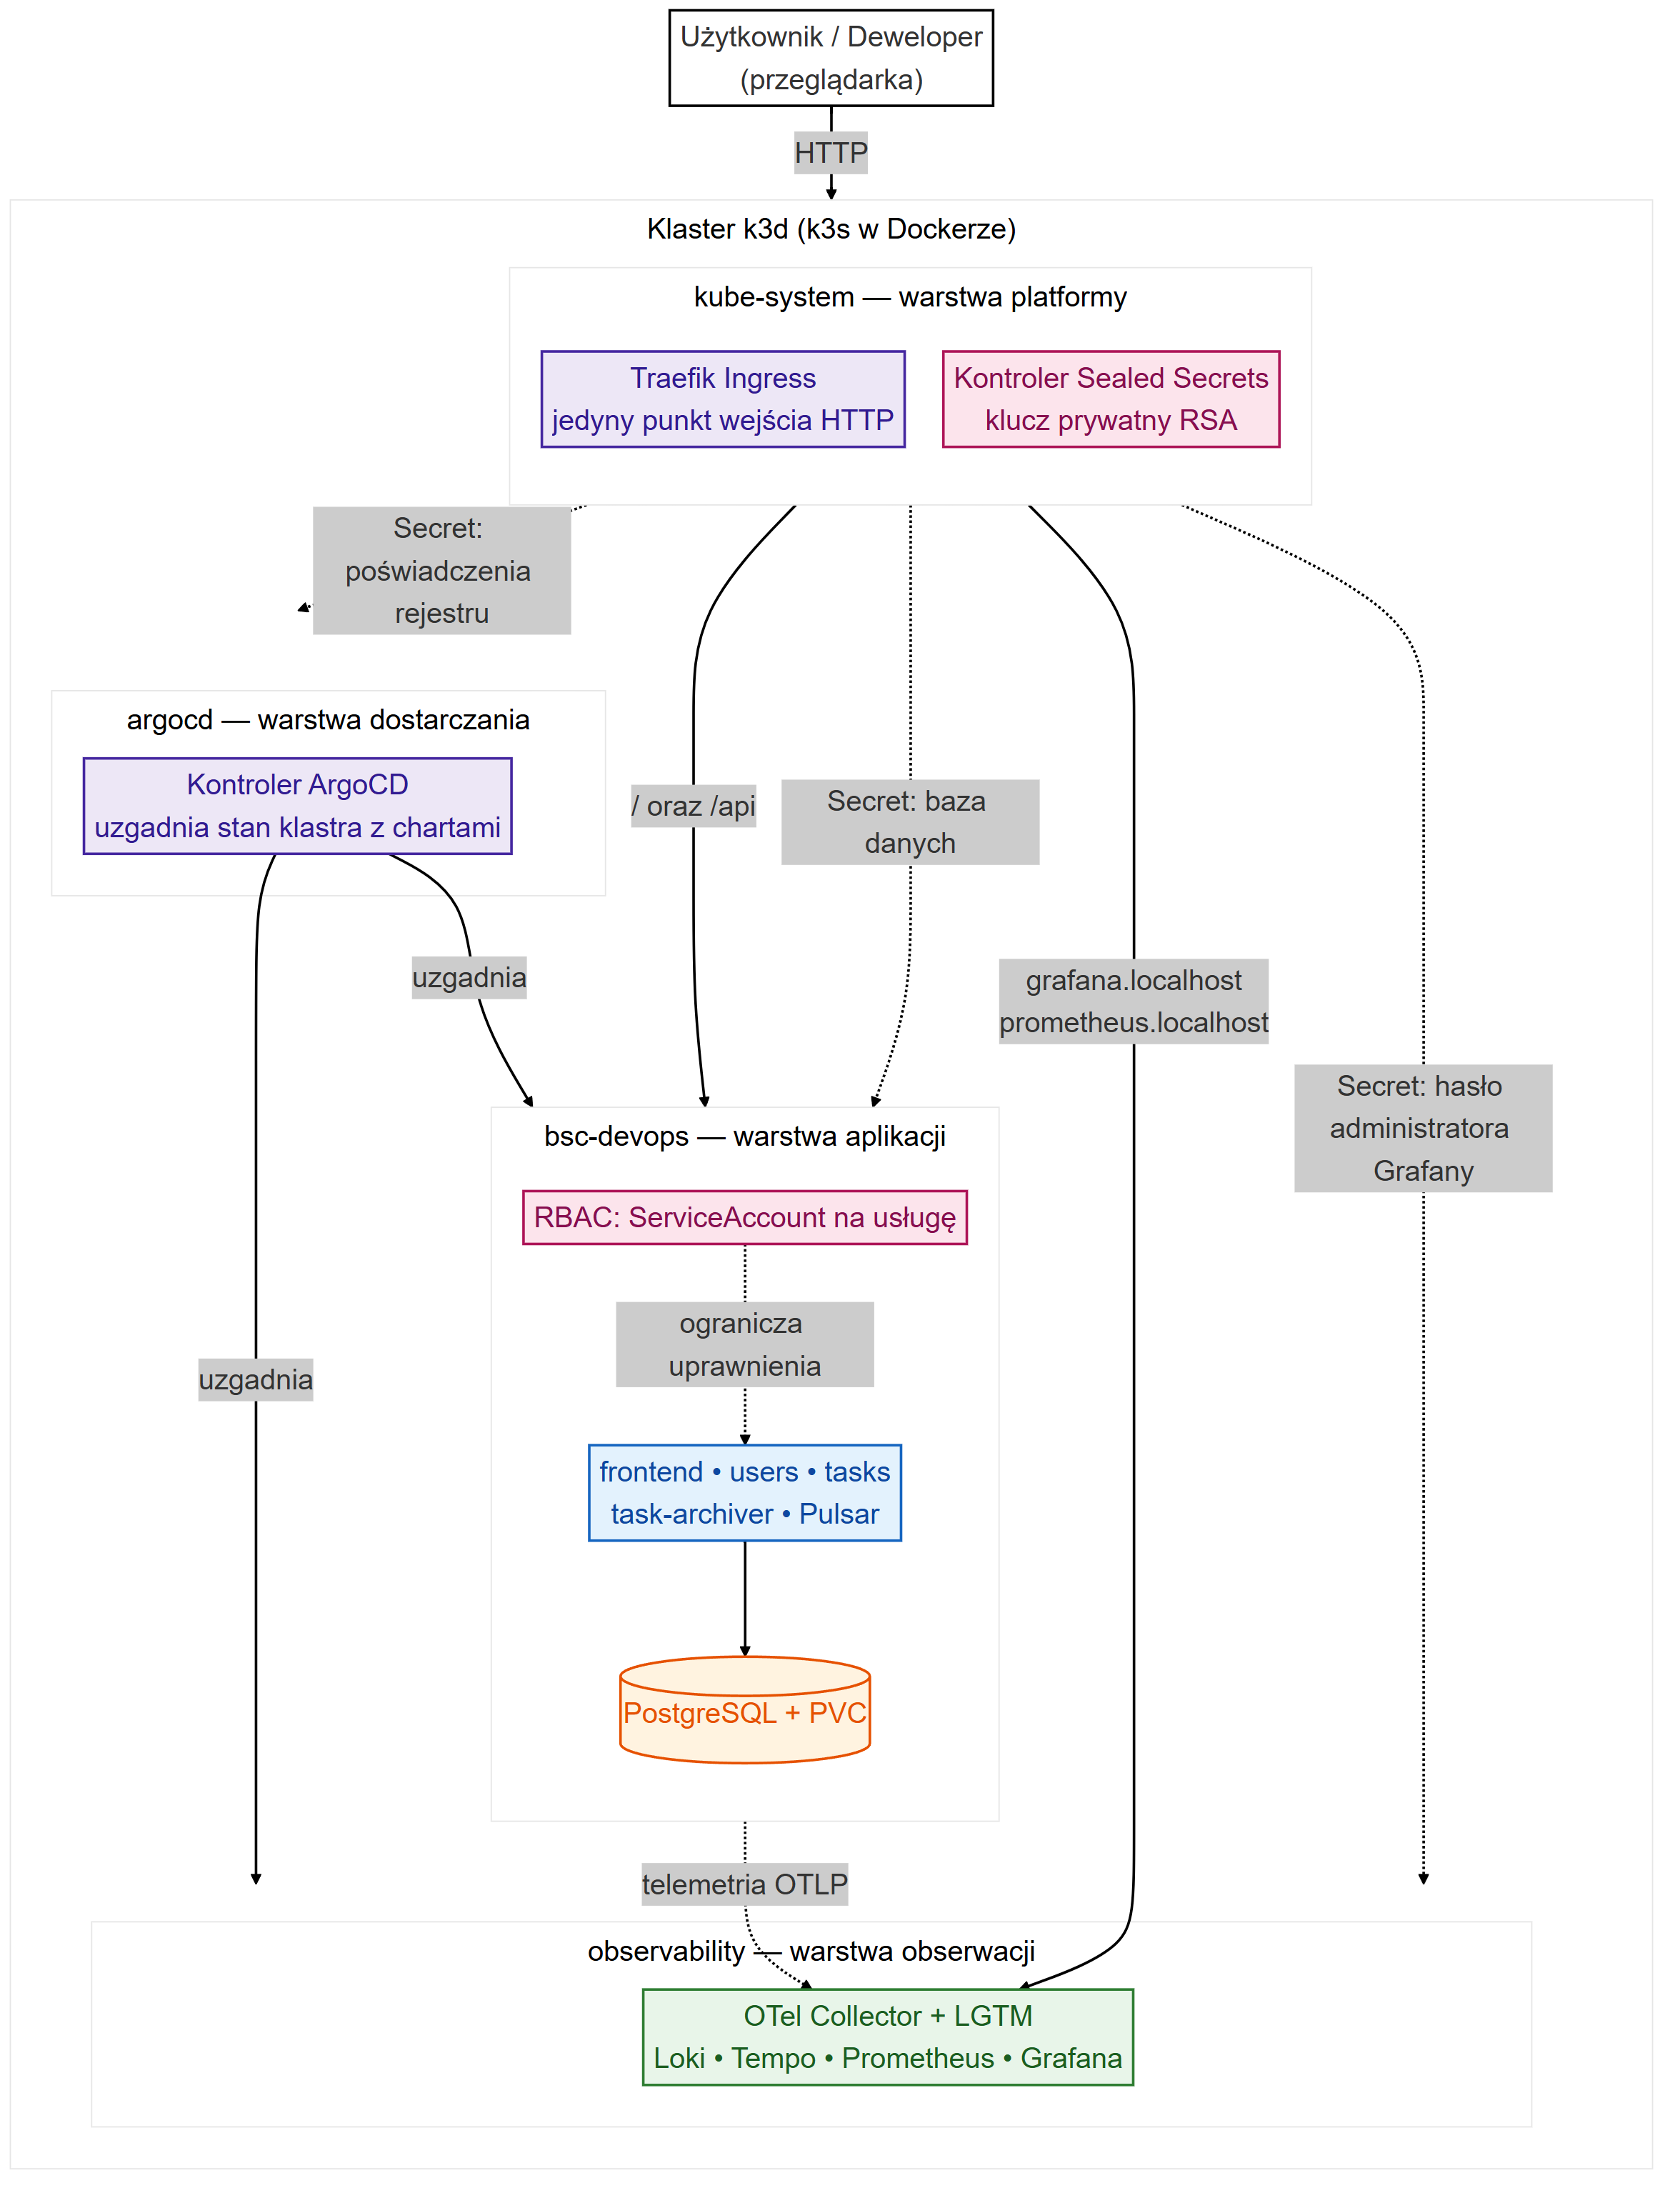
\includegraphics[width=0.95\textwidth]{img/diagrams/08-operate/operate-01-infrastructure.png}
    \caption{Infrastruktura klastra --- cztery przestrzenie nazw, cztery role: platforma, dostarczanie, aplikacje i~obserwacja; kontroler Sealed Secrets odszyfrowuje sekrety do trzech przestrzeni (opracowanie własne).}
    \label{fig:infrastructure}
\end{figure}

\subsubsection{Usługi wspierające w~klastrze}
Zgodnie z~założeniem o~pełnej odtwarzalności środowiska w~modelu lokalnym, zdecydowano się na uruchomienie odpowiedników usług chmurowych bezpośrednio wewnątrz klastra Kubernetes przy użyciu gotowych chartów Helm.
\begin{itemize}
    \item \textbf{Baza danych: PostgreSQL (zamiast AWS RDS):} Dane mikroserwisów są przechowywane w~relacyjnej bazie danych PostgreSQL. W~klastrze lokalnym baza ta działa jako kontener z~zamontowanym wolumenem trwałym (ang. \textit{Persistent Volume}), co zapewnia trwałość danych mimo restartów kontenerów.
    \item \textbf{Broker wiadomości: Apache Pulsar (zamiast np. Amazon MSK):} Komunikacja zdarzeniowa między mikroserwisami odbywa się przez tematy brokera Apache Pulsar uruchomionego w~klastrze; w~środowisku chmurowym rolę tę przejęłaby usługa zarządzana.
\end{itemize}

Ten sam wzorzec zastępowania dotyczy pozostałych elementów platformy. Rysunek~\ref{fig:aws-equivalent} zestawia komponenty uruchomione lokalnie z~ich zarządzanymi odpowiednikami w~chmurze AWS --- wariant chmurowy pozostaje propozycją, świadomie niezaimplementowaną w~ramach pracy, ilustrującą jednak niezależność platformy od konkretnego dostawcy.

\begin{figure}[H]
    \centering
    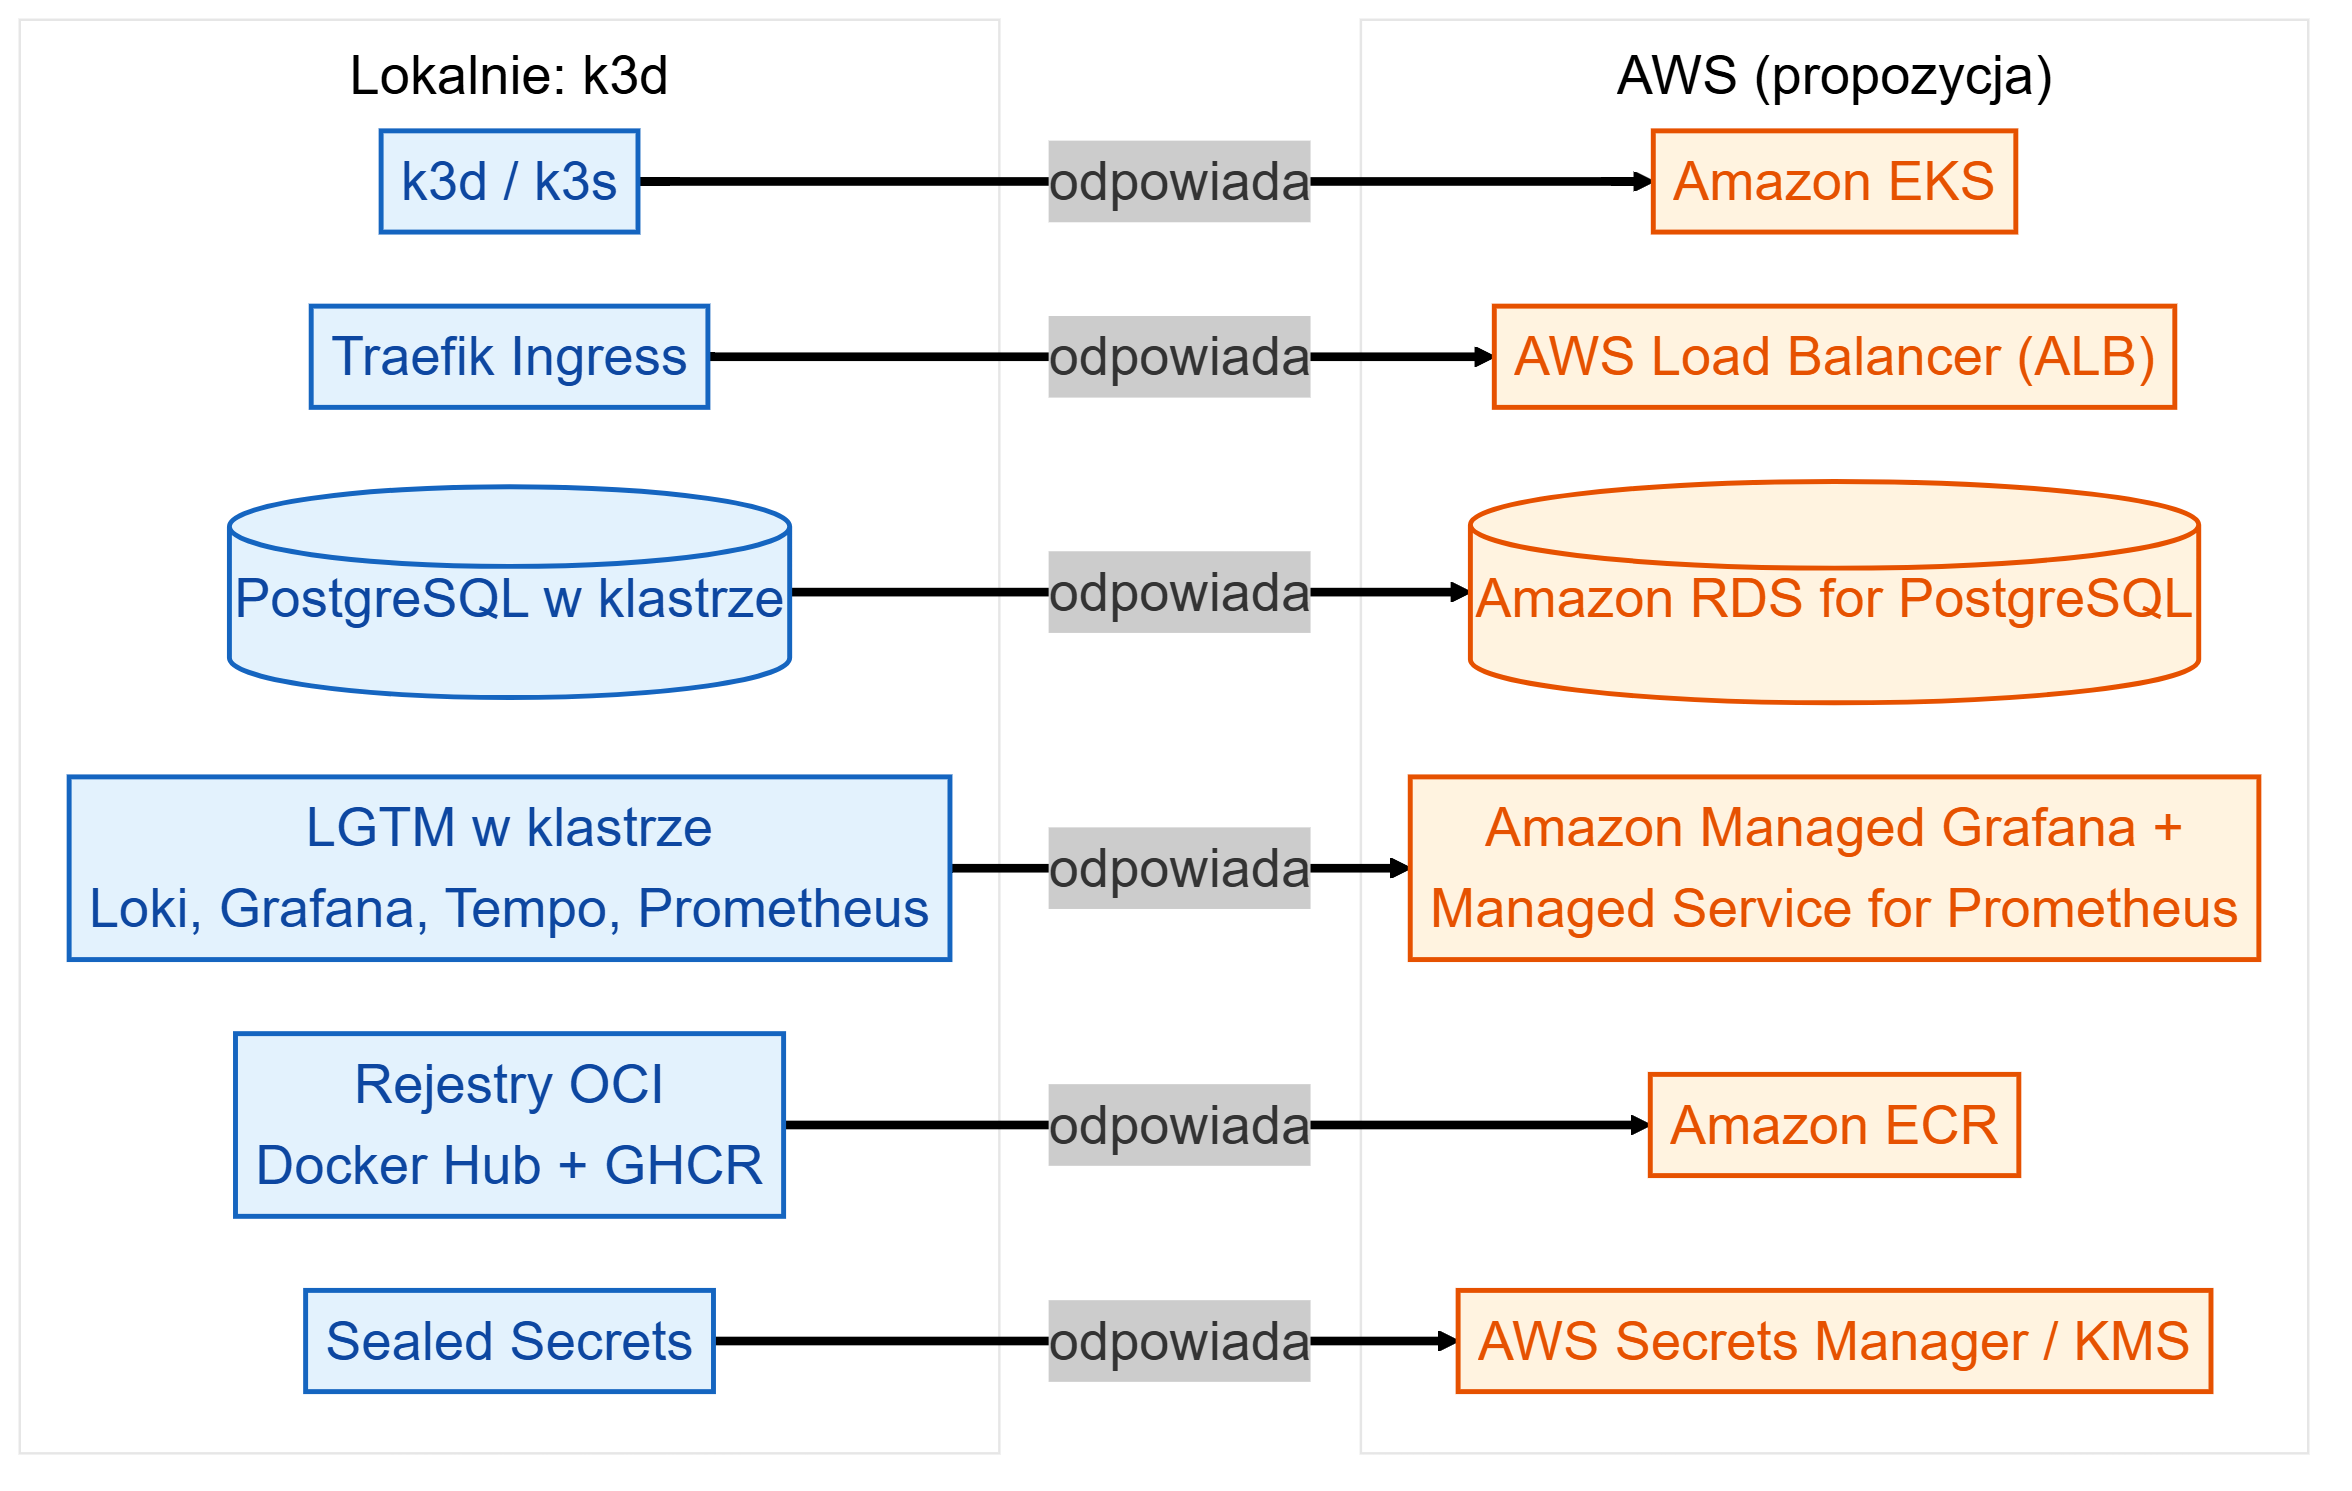
\includegraphics[width=\textwidth]{img/diagrams/08-operate/operate-02-aws-equivalent.png}
    \caption{Mapowanie lokalnego środowiska na zarządzane usługi AWS --- propozycja migracji ilustrująca niezależność od dostawcy; wariant chmurowy nie był implementowany (opracowanie własne).}
    \label{fig:aws-equivalent}
\end{figure}

\subsubsection{Zarządzanie zasobami: Kubernetes}
Kubernetes zarządza cyklem życia wszystkich komponentów, dbając o~ich samonaprawę (ang. \textit{self-healing}) oraz odpowiednie przydzielanie zasobów procesora i~pamięci. Wykorzystanie lokalnego klastra pozwala na demonstrację tych mechanizmów bez generowania kosztów infrastrukturalnych.
